\documentclass{article}
\usepackage{ctex}
\usepackage{graphicx}
\usepackage{amsmath}
\usepackage{indentfirst}
\usepackage{titlesec}
\usepackage{setspace}
\usepackage{subfigure}
\usepackage{caption}
\usepackage{float}
\usepackage{booktabs}
\usepackage{geometry}
\usepackage{multirow}
\geometry{left=1.2cm,right=1.2cm,top=2cm,bottom=2cm}
\title{\songti \zihao{2}\bfseries 闪烁体荧光衰减长度测量预习报告}
\titleformat*{\section}{\songti\zihao{4}\bfseries}
\titleformat*{\subsection}{\songti\zihao{5}\bfseries}
\renewcommand\thesection{\arabic{section}}
\author{王启骅 PB20020580}
\begin{document}
	\maketitle
	\section{实验目的}
	1. 了解塑料闪烁计数器的一般结构、性能和应用。
	
	
	2. 初步了解一种测量长塑料闪烁体技术衰减长度的方法。
	
	\section{实验装置}
	单道闪烁能谱仪一套;
	长塑料闪烁体一块(带探头);
	90Sr—90Yb 放射源一个;
	示波器一台。
	
	\section{实验原理}
	塑料闪烁体是在苯乙烯溶液中加入对联三苯(第一溶质)和 POPOP(第二溶质)聚合
	而成。当带电粒子射入塑料闪烁体时,先使苯乙烯分子激发,在猝灭前把激发能转给第一溶
	质对联三苯分子,其发光衰减时间约为 10-9
	s 。当第一溶质激发态的分子退激时发出的光几
	乎全部被第二溶质所吸收,后者以同样量级(~10-9
	s)的发光衰减时间退激,然而发出光的波
	长是比前者长的可见光或紫光(3500~4800Å),能与光电倍加管的光阴极光谱响应配合得更
	好。
	
		\begin{figure}[!h]
		
		\centering
		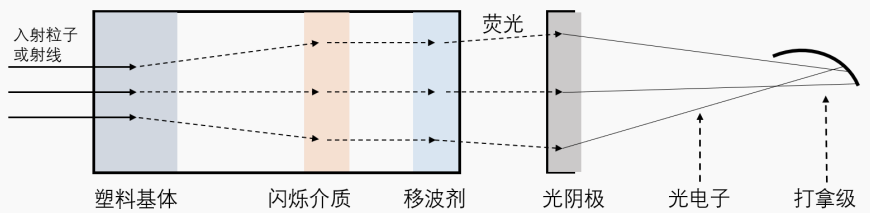
\includegraphics[scale=0.7]{原理}
		\captionsetup{font={small},labelfont=bf}
		\caption{\heiti\zihao{-5}塑料闪烁体原理}
		
	\end{figure}


塑料闪烁体的光传输性能不仅依赖闪烁体本身的性质和几何结构,而且与闪烁体表面的
抛光程度,包复物的反光情况等都有很大关系。因此塑料闪烁体的技术衰减长度为 50cm—
100cm。


在塑料闪烁体中,产生的光到达收集光的光电倍增管要经过多次散射。光通过闪烁体和
光导的透射率随通过的距离按指数规律衰减。即光强度
\begin{equation}
	I=I_0\exp(-\mu x)
\end{equation}


其中 I0 为射线在闪烁体中产生的光强度,I 为光在闪烁体中传输了长为 x(cm)距离的光
强度,μ是光在闪烁体和光导中的吸收系数。通常我们是以吸收系数的倒数 1/μ定义为闪烁
体的技术衰减长度(1/cm),也就是当光强度衰减到原强度的 1/e 时的闪烁体长度为技术衰减
长度。应该指出,这里所谓技术衰减长度 1/μ 是对在闪烁体中的各种波长光的有效技术衰
减长度,因为实验中我们没有用任何的波长过滤器。


这些经塑料闪烁体和光导衰减后的光被光电倍增管的光阴极所收集并转换成光电子,后
者经电子倍增后到达阳极,使阳极负载电阻上有个电压脉冲 V 输出。如果从收集光到产生
一个输出幅度 V 的电压脉冲的各种过程都是线性的,也就是说输出电压脉冲幅度 V 正比于
光阴极所收集到的光子强度 I 即 V = kI。其中 k 为常数。因此

\begin{equation}
	V=V_0\exp(-\mu x)
\end{equation}


该实验测量有效技术衰减长度的装置方框图为图 2 所示。根据(2)
式,具体测量方法是采用 $ ^{90}Sr—^{90}Yb $ 的β放射源与闪烁体表面保持固定距离,平行于闪烁体
移动源,改变源与闪烁体一端(近光阴极一端)的距离 x,对应不同 x 值相应的测出积分计
数为一定值(如减去本底后的纯计数为 5000 个脉冲)的单道分析器的甄别阈值 V,以 x(cm)
为横坐标,甄别阈值 V 为纵坐标在半对数坐标纸上即可得到光传输性能曲线,直线部分斜
率的倒数即为有效技术衰减长度。
	\begin{figure}[!h]
	
	\centering
	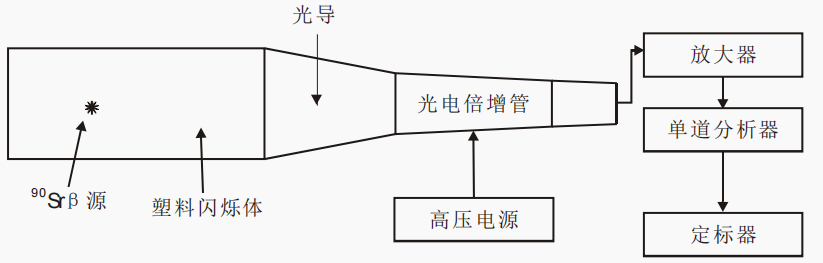
\includegraphics[scale=0.7]{原理2}
	\captionsetup{font={small},labelfont=bf}
	\caption{\heiti\zihao{-5}长塑料闪烁体技术衰减长度测量装置}
	
\end{figure}

\section{实验步骤}
1. 探头检查
用黑布将整个闪烁计数器包住,联结仪器,接通电源,经检查无误后方可打开高压电源
开关预热 1—2 分钟,打开高压开关(注意此时高压不能调得太高,为什么?),开定标
器,逐步掀开黑布,观察本底计数有无明显增加。若无明显增加,说明闪烁计数器光密
封性能好。否则,应立即关闭高压,找出漏光部分,用黑胶带重新密封,重新检查漏光,
直到整个黑布去掉后本底计数没有明显增加为止。


2. 用脉冲示波器观察并测量光电倍增管输出电压脉冲的前沿。


3. 测量有效技术衰减长度,要求各点的积分计数相对统计误差小于 1.5%,测出不同 x 值
所对应的甄别阈值 V(伏)。

\section{数据处理}
参考放射性核素 $ ^{116m }$
In 的半衰期测定实验讲义中的最小二乘法原理。根据实验所测量到
的$ x_i $和$ V_i $的数据,利用最小二乘法原理求出实验数据的拟合曲线和计算有效技术衰减长度。
\end{document}